\documentclass{report}
\usepackage{url}

\usepackage[left=1in, right=1in, top=1in, bottom=1in]{geometry}
\usepackage{float}
\usepackage[]{graphicx}
\usepackage{subfigure}
\graphicspath{{./graphics/}}
\usepackage{lipsum}

\usepackage{listings}
\usepackage{color}
\usepackage[usenames,dvipsnames]{xcolor}

\definecolor{dkgreen}{rgb}{0,0.6,0}
\definecolor{gray}{rgb}{0.5,0.5,0.5}
\definecolor{mauve}{rgb}{0.58,0,0.82}

\lstset{frame=none, %tb
  language=C,
  aboveskip=3mm,
  belowskip=3mm,
  showstringspaces=false,
  columns=flexible,
  basicstyle={\small\ttfamily},
  numbers=left,
  numberstyle=\tiny\color{gray},
  keywordstyle=\color{blue},
  commentstyle=\color{OliveGreen},
  stringstyle=\color{mauve},
  breaklines=true,
  breakatwhitespace=true,
  tabsize=3
}

\begin{document}

\begin{titlepage}
\begin{center}
  \bfseries
  \huge UNIVERSITY OF YORK
  \vskip.1in
  \bfseries
  \large Department of Computer Science
  \vskip2in
  \huge Implementing MrsP on Fully Partitioned Systems
\end{center}

\vskip1in

\begin{minipage}{.25\textwidth}
  \begin{flushleft}
    \bfseries\large Author:\par Shuai Zhao
  \end{flushleft}
\end{minipage}
\hskip.4\textwidth
\begin{minipage}{.25\textwidth}
  \begin{flushleft}
    \bfseries\large Supervisor:\par Andy Wellings
  \end{flushleft}
\end{minipage}

\vskip1.3in

\centering
\bfseries
\Large \today
\end{titlepage}


\begin{abstract}
Compared to the matured and well-designed resource sharing solutions on uniprocessor systems, resource sharing protocols on multiprocessor systems are usually complex and more difficult to deploy in a standard real-time system. Among the existing multiprocessor resource sharing protocols, there is a schedulability analysis compatible multiprocessor locking protocol named MrsP. As MrsP introduces job migrations as a helping mechanism, implementing such a protocol inside a kernel can introduce considerable complexity to the system, especially for fully partitioned ones. In this report we investigate and explore possible implementation solutions of MrsP under fully partitioned systems with fixed priorities. We mainly focus on the feasible implementation approaches of the migration-based helping mechanism with identified issues and challenges. Three different kernel-supported approaches are presented and discussed with their unique advantages and limitations. In addition, we also provide an outside-kernel MrsP implementation under generic Linux. 
\end{abstract}

\tableofcontents

\chapter{Introduction}
\label{Section_Introduction}
Resource sharing problems when concurrent or parallel tasks access the same resource. If not handled correcting the access can result in corrupt data or deadlocks.
On uniprocessor systems, matured resource sharing protocols exist are well-practiced over decades to provide safe access with minimum blocking times. In the last few years, the increasing demand of computation power leads to a trend of transiting from uniprocessor to multiprocessors platforms. On multiprocessor systems, tasks are able to access a shared resource in parallel, which breaks the existing resource sharing protocols for uniprocessor systems as they does not handle resources that can be accessed from different partitions. Unfortunately, technology for resource sharing on multiprocessor systems is much less matured than in uniprocessor systems. Although there exist several multiprocessor locking protocols, they either carry strong constraints e.g. no support for nested access or high run-time overheads with a poor schedulability support. In addition, in practice, protocols for multiprocessors are usually complex and have a high implementation difficulty. 

Among the existing multiprocessor locking protocols, MrsP is the first protocol proposed to be compatible with Response Time Analysis~\cite{audsley1993applying} by proposing an elegant helping mechanism. Compared to other protocols, MrsP theoretically removes the restriction of nested resource access and is able to bound the blocking of a task that requests a resource to $O(m)$, where $m$ indicates the number of processors that have tasks requesting the same resource [8, 10], and can outperforms protocols with either the non-preemptive or priority ceiling approaches. The original MrsP proposal proposes two possible approaches to realise the helping mechanism. For a stateless resource, a duplicated execution approach can be applied so that the waiting task takes over the work of the resource holder and executes the critical section on its behalf. However, in the more general case, migrations are needed. Once a resource holder is preempted, it can migrate to a partition that has a task spinning for the same resource. However, such a migration-based helping mechanism can introduce a considerably high complexity to the MrsP implementation, especially when an in-kernel implementation is required.

In this report we aim to investigate and explore feasible approaches to realise the migration-based helping mechanism. We mainly focus on the implementation inside the kernel but will provide an outside-kernel implementation as well. The in-kernel MrsP implementations are built inside the Preemptive Fixed-Priority (P-FP) scheduler of the Litmus kernel~\cite{calandrino2006litmus, brandenburg2011scheduling}, while the outside-kernel version is implemented under generic Linux. In addition, the advantages and limitations of each implementation is discussed and presented in this report. All implementations can be accessed via link: \emph{https://github.com/zs673/litmus\_mrsp}.

The remainder of this report is divided into 6 chapters. Chapter \ref{MrsP Review} provides a review of MrsP. Chapter \ref{litmus} gives a description of Litmus, where the in-kernel MrsP implementations are built on. The design and implementation of the in-kernel MrsP infrastructure is described in Chapter \ref{MrsP Infrastructure}. Chapter \ref{Migration-based Helping Mechanism} describes the design and implementation details of three approaches to build the in-kernel MrsP helping mechanism. Chapter~\ref{Out Kernel} provides a description of an outside-kernel MrsP implementation under generic Linux. Finally, conclusions are presented in Chapter \ref{Conclusion}.



\chapter{MrsP}
\label{MrsP Review}
MrsP (proposed in~\cite{burns2013schedulability}) is the first multiprocessor locking protocol for partitioned fixed-priority systems that is compatible with the uniprocessor Response-Time Analysis (RTA) framework~\cite{audsley1993applying} with minors modification to reflect potential parallel access to global resources. Under MrsP, the maximum blocking time that a resource-requesting task can suffer is bounded by the number of processors that have tasks requesting the same resource. The creation of MrsP is inspired by SRP with fixed priority systems: spin locks are adopted and resources are served in a FIFO order. However, \cite{burns2013schedulability} argues that spinning non-preemptively leads to poor schedulability as each highest-priority task needs to deal with the longest blocking time on its processor;  therefore, the paper proposes that tasks under MrsP should only spin at the local ceiling priority. With this principle, MrsP defines the following basic rules:
\begin{itemize}
\item Each resource is assigned with one resource ceiling priority for each processor that contains tasks requesting the resource. The resource ceiling is defined to be the highest priority among the local tasks that request the resource.
\item Tasks raise their priorities to the resource ceiling immediately once they attempt to lock the resource. 
\item If the resource is unavailable, the task should spin on its processors with the corresponding ceiling priorities and wait in a FIFO order.
\end{itemize}

These rules set a fixed maximum length of the FIFO queue, which is the number of processor that contains tasks that request the resource. However, spinning at the local ceiling level can lead to a prolonged blocking time as the resource holder can be preempted by higher priority local tasks. To match RTA, a helping mechanism is introduced to help the preempted resource holder. This is defined as follows:
\begin{itemize}
\item A task that is waiting for a resource should be capable of executing the critical section on behalf of any other tasks that are waiting for the same resource.
\item The helping task should undertake the computations of other waiting tasks based on the FIFO queuing order.
\end{itemize}

The helping mechanism allows tasks to help the preempted resource holder to make progress by using the wasted cycles instead of spinning uselessly. In the worst case, a resource requesting task should execute all the computations of tasks in the FIFO queue each time when it tries to access the resource, which leads to a worst case blocking time of the length of the FIFO queue multiplied by the cost for accessing the resource. With the helping mechanism, MrsP matches with the RTA equation (\ref{eq1}) and (\ref{eq2}).

\begin{equation} \label{eq1}
R_{i}= C_{i}+ max\left \{ \widehat{e},\widehat{b} \right \} + \sum_{\tau _{j} \in hpl(i) }\left \lceil  \frac{R_{i}}{T_{j}}   \right \rceil C_{j} 
\end{equation}

\begin{equation} \label{eq2}
C_{i}=WCET_{i}+\sum_{r^{j}\in F(\tau _{i})}n_{i}e^{j}
\end{equation}

As shown in equation (\ref{eq1}), the response time $R_{i}$ for task $i$ is decided by its execution time $C_{i}$, the maximum blocking time and 
the interference from higher-priority tasks, where $\widehat{e}$ is the maximum execution time of resources that are used by low priority tasks and at least one equal or higher priority task; $\widehat{b}$ is the maximum time of non-preemptive sections incurred by the operating system; and $hpl(i)$ indicates a set of high priority local tasks. $C_{i}$ can be further decided by the worst-case execution time of $T_{i}$ without resources and the time it spends with each resource with serialization effects, see equation (\ref{eq2}), where $r^{j}\in F(\tau _{i})$ gives a set of tasks that use resource $j$ and $n_{i}$ is the number of times $\tau _{i}$ uses the resource. To reflect potential parallel access for resources, the entity $e_{j}$ is introduced to represent the full execution time of a resource. With MrsP, this value can be bounded by the number of processors that contain tasks request the resource due to the adopting of FIFO spin and the helping approach. Therefore, MrsP can fit into the RTA and is a optimal multiprocessor locking protocol as the blocking of a task is bounded by the number of processors m (i.e. $O(m)$) ~\cite{brandenburg2010optimality}. In addition, MrsP guarantees deadlock free and support nested resource access by assigning locks with orders. A safe upper bound execution time for accessing nested resources is provided as well.

\chapter{Litmus\textsuperscript{RT}}
\label{litmus}
The Linux Testbed for Multiprocessor Scheduling in Real-time Systems~\cite{calandrino2006litmus, brandenburg2011scheduling} is a real-time patch to the Linux kernel. Litmus is a configurable testbed for researching scheduling schemes and synchronization algorithms. By hooking into the Linux scheduling framework, Litmus overrides the scheduling decisions made by Linux and provides its own dispatching policies. It then provides a plugin interface that allows users to define various scheduling policies with locking protocols. Litmus\textsuperscript{RT} is built with four components: core infrastructure, scheduler plugins, user-space API, user-space Library and tools, as shown in Figure~\ref{litmusxx}. The core infrastructure connects to the scheduling algorithm of Linux kernel and allows the use of the Litmus scheduling plugins with customization. The scheduling plugins contain the implementations of various dispatching policies with locking protocols in a modular style and is statically compiled with the Kernel. During runtime, these plugins can be switched dynamically.

\begin{figure}[h]
\centering
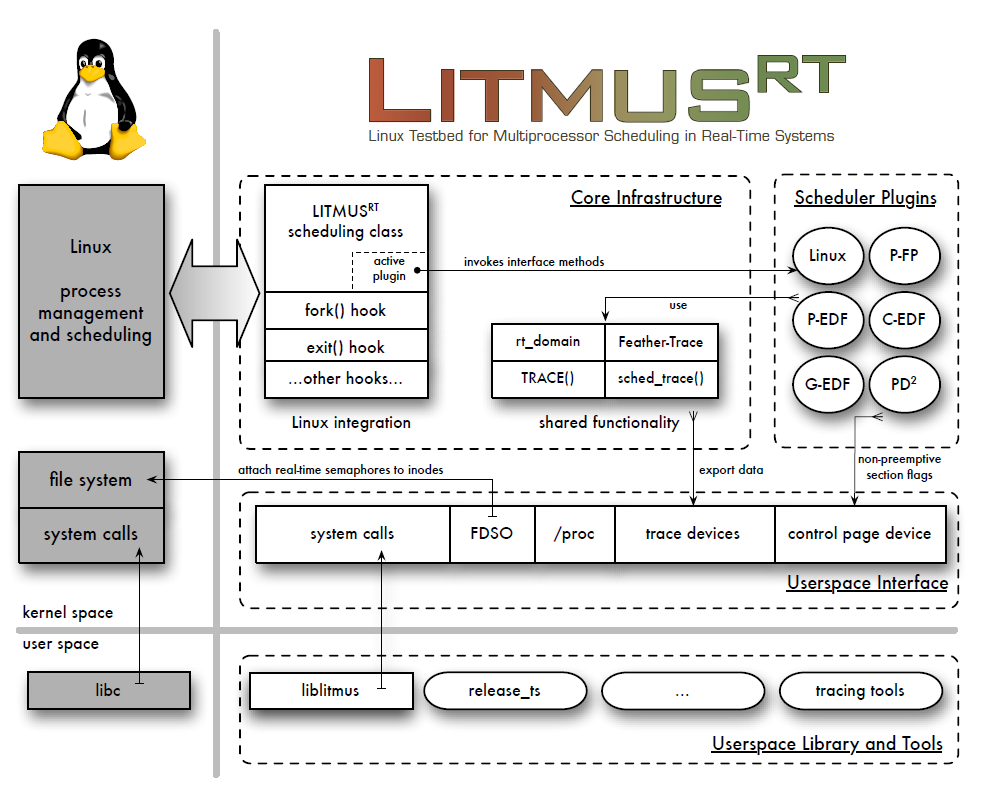
\includegraphics[width=.8\columnwidth]{graphics/litmus.png}
\caption{Litmus\textsuperscript{RT} Structure.}
\label{litmusxx}
\end{figure}

In this report we focus on a fully partitioned system with fixed priority (P-FP). As with Linux, the P-FP scheduler in Litmus maintains a priority ordered run queue structure for each processor and each run queue is protected by a local spin lock. With P-FP scheduling selected, Linux will forward the scheduling requests to Linux through the function \texttt{litmus\_schedule()}, which further forwards the request to P-FP scheduler by invoking its function \texttt{schedule()}. Basically, the \texttt{schedule()} function saves the previous scheduled task based on its status and then returns the highest priority task in the run queue on that processor to schedule. After a scheduling decision is made, the function \texttt{finish\_switch()} will be invoked to handle the situation where the previous scheduled task needs to migrate due to a locking protocol decision by simply placing the task into a remote run queue. Inside the scheduling class, locking protocols can be implemented and behaviours can be defined via the  \texttt{lock()} and \texttt{unlock()} interfaces.

\begin{figure}[h]
\centering
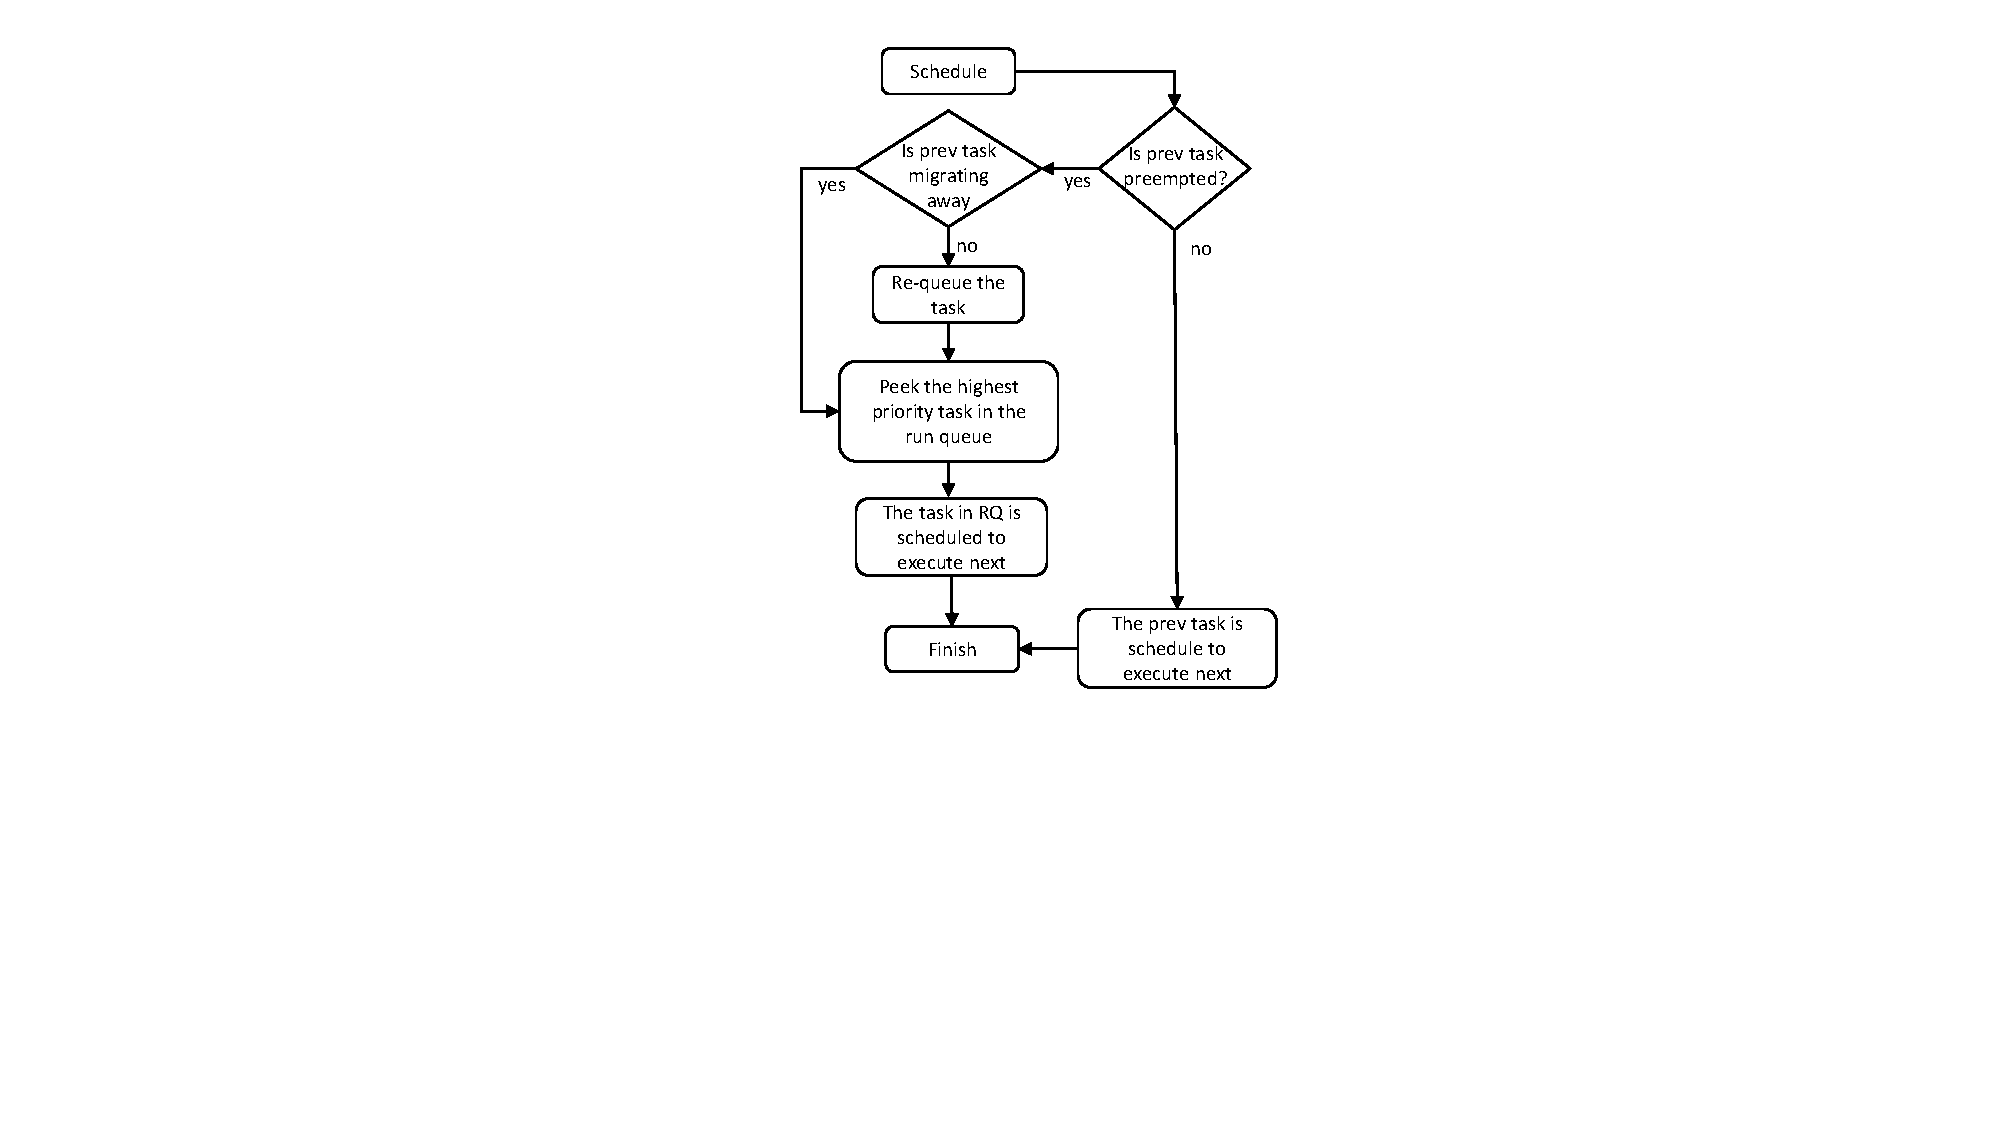
\includegraphics[width=.6\columnwidth]{graphics/pfp1.pdf}
\caption{P-FP scheduling routine in Litmus\textsuperscript{RT}.}
\label{pfp}
\end{figure}

The scheduling routine of the P-FP scheduler is illustrated in Figure~\ref{pfp}. For each partition, the P-FP scheduler maintains a ready queue and a sleeping queue. Upon each scheduling point, the scheduler first checks whether the current scheduled task (1) will be preempted by a higher priority task in the ready queue; (2) needs to migrate to a remote partition; (3) exhaust its budget or (4) is going to sleep. The scheduler inserts the scheduled task into either the ready queue or sleeping queue based on the status of the task except in the migration case. Then the scheduler looks into the ready queue and returns with the highest priority task (if any) to be scheduled next. If the previous scheduled task is not preempted, the scheduler simply returns and keeps executing the task. The function \texttt{finish\_switch()} will be invoked after the \texttt{schedule()} function returns to handle the migration of the previous scheduled task by inserting it into the corresponding remote ready queue.

\chapter{MrsP -- Infrastructure}
\label{MrsP Infrastructure}
This chapter describes the MrsP infrastructure, which consists of two major components: FIFO spin locks and resource ceilings. Although the infrastructure can be built via various approaches, we will only describe one in this report as we mainly focus on the helping mechanism. In~\cite{mezzetti2015challenges}, more options to build the FIFO ordering and spinning are presented and discussed. The implementation of the infrastructure for all in-kernel MrsP implementations are identical.

\section{FIFO spin locks}
The FIFO spin locks are modelled via a linked list. Under MrsP, each resource has a lock structure associated with a \emph{head} task to indicate the first requesting task as well as a \emph{tail} to track the last task in the requesting queue. In addition, each task holds a reference to the next resource-requesting task (if any). Once a task requests a resource, it will be placed into the list with a FIFO order. A task will be granted with the resource only if it becomes the head of the requesting queue. The following pseudo code illustrates this approach. 

\begin{lstlisting}
struct task{
	task *next;
}
struct mrsp_lock_struct {
	task *head;
	task *tail;
	int  *priority_per_processor;
}
void mrsp_lock(struct mrsp_lock_struct* lock){
	... // code for priority raising.
	atomic{
		CURRENT_TASK->next = NULL;
		if(head == NULL)
			lock->head = lock->tail = CURRENT_TASK;
		else
			lock->tail->next = CURRENT_TASK;
	}
	while (1){
		if(lock->head == CURRENT_TASK)
			break;	
	}
}
void mrsp_unlock(struct mrsp_lock_struct* lock){
	atomic{
		if(lock->head->next != NULL){
			lock->head = lock->head->next;
		}
		else{
			lock->head = lock->fail = NULL;	
		}
	}
	... // code for priority restoring.
}
\end{lstlisting}

Upon a resource request, the task will check whether the FIFO queue is empty. If so, it becomes the \emph{head} (as well as the \emph{tail}) and is able to lock the resource. Otherwise, it is placed into the list as the \emph{tail} and spins inside the while loop. Once the holder releases the resource, it sets the next task (if any) in the list as the \emph{head}, which is then able to break the loop and lock the resource.  Kernel spin locks are used in the non-preemptive sections inside the function \texttt{lock} and \texttt{unlock} e.g. when modifying the FIFO queue.

\section{Resource Ceilings}
The ceiling priorities for a resource is defined during the initialization phase of a MrsP lock as an array of ceilings, one for each on-line processor, and passed to kernel space through function \texttt{open\_mrsp\_sem()}, which eventually invokes the MrsP lock initialization function \texttt{new\_MrsP()}. The ceiling priorities will be stored by the pointer \texttt{priority\_per\_processor} in the \texttt{mrsp\_lock\_struct}. Meanwhile, each resource-requesting task will take a copy of the resource ceiling of its original partition when entering the \texttt{lock} function to avoid a frequent access to the ceiling array. 

During accessing a MrsP resource, a priority change will be triggered:
\begin{itemize}
\item when a task enters into the \texttt{lock} function, it raises its priority to the ceiling on its processor immediately i.e. before adding itself to the FIFO queue;
\item before returning from \texttt{unlock} function, a task restores its priority to the original one;
\item a task updates its priority to the ceiling on the current processor immediately after each migration;
\item upon each migration due to helping, the resource holder inherits the priority of the spinning task (the corresponding resource ceiling on the partition) before it resumes;
\item when migrating back to its original processor due to a nested preemption, the holder simply updates its priority to the corresponding resource ceiling based on the ceiling it stored when entering the \texttt{lock} function.  
\end{itemize}

\chapter{MrsP -- Migration-based Helping Mechanisms}
\label{Migration-based Helping Mechanism}
In this section, three feasible approaches for implementing the migration-based helping mechanism inside Litmus kernel are presented and discussed. The Generic Linux Migration Approach (Mrsp-generic) is commonly adopted while realizing the helping mechanism. Such an approach is straightforward during design and implementation but can suffer from race conditions between run queues, which either triggers superfluous migrations or fails to trigger a necessary migration. In this report we refer such migration failures as \emph{false migrations}. The task swapping approach (MrsP-swapping) is a novel approach for building the helping mechanism, where the resource holder swaps with a task spinning for the same resource (if any) upon each preemption. The task swapping approach carries the advantage of being scheduler-modifications free (i.e. in the viewpoint of implementation, the helping mechanism can be modelled as a part of the protocol rather than the scheduler). However, the swapping approach brings a considerably high complexity to the implementation, especially on \emph{nested preemption} cases, where the resource holder is preempted again on a remote partition. The Preemption Queue With Non-Preemptive Sections (MrsP-NP) approach aims to improve the efficiency of the helping mechanism by avoiding the false migrations mentioned above as well as the \emph{frequent migrations}, where the resource holder is preempted immediately after a migration.

\section{Generic Linux Migration Approach (MrsP-Generic)}
In the generic Linux kernel, cpu masks are provided to built global, partitioned and clustered scheduling under multiprocessors via task affinities. In the fixed priority scheduler, task migrations are handled by a set of push and pull operations, as part of the scheduling routine. We use $P_{t}$ to denote the target processor, $P_{s}$ to denote the source processor and $RQ_{i}$ to denote the run queue of processor $i$. The push operation is performed after a scheduling decision. This will push (i.e. place the task into $RQ_{t}$) a queued local task to $P_{t}$ if the affinity set of the task contains $P_{t}$ and the task has the highest priority on $P_{t}$. Once a task is preempted or resumed, Linux triggers the push operation up to three attempts in order to migrate the task to a suitable processor. If this fails, the task will not be considered again and scheduling the task relies on pull operations. A queued task can be pulled from $P_{t}$ if the task is not assigned to $P_{t}$, $P_{t}$ is included in the task affinity, and the task has the highest priority on $P_{t}$. The pull operation triggers every time before the scheduling decision point when the to-be-scheduled task has a lower priority than the previous scheduled task. The pull operation will check all remote run queues based on a increasing order of CPU indices to identify a suitable task to migrate~\cite{bovet2005understanding}.

While implementing the MrsP helping mechanism inside a fully partitioned scheduler without a migration facility, the most straightforward approach is to built a simple and restricted version of Linux migration model. While a task is preempted with a MrsP resource, the scheduler forwards the task to \texttt{finish\_switch} function, where the push operation is initiated. The push operation aims to migrate the task to a processor with a task spinning for the same resource. To preempt the spinning task, the migrated task will be assigned with a priority sightly higher than the corresponding ceiling. The push operation first inserts the task into the run queue of the processor which contains the first waiting task and then checks whether the preempted task has the highest priority on the processor. Once the requirements are satisfied, the preempted task will be assigned to the target processor and waits to be scheduled by the remote scheduler. Otherwise, the attempt fails and system will try to push the task to another valid processors based on the FIFO waiting order. Upon a nested preemption i.e. preempted again after migration, push operation checks whether the original processor is valid to execute on before it looks into processors with a spinning task.

The pull operation is implemented inside the while loop in the \texttt{lock} function and is triggered every time the resource holder is queued in a remote processor. Accordingly, a waiting task continuously checks the status of the resource holder as long as it is executing. If the resource holder is preempted, the holder will be replaced in the local run queue with a slightly higher priority and the processor reassigned. Then the pull operation checks again whether the migrated task holds the highest priority in local run queue. If so, the pull operation returns with a explicit call to \texttt{schedule} so that the resource holder can preempt the spinning task and execute. In the case where the resource holder resumes itself or a higher priority task is queued in the local run queue, the pull operation returns with a failed attempt. The following pseudo code illustrate the routine of MrsP pull operation.

\begin{lstlisting}
/* If the holder is currently preempted */
if(atomic_read(&sem->lock_holder_preempted) == 1){
	struct task_struct *head = sem->head;

	/* take the holder out of the current ready queue */
	atomic{
		fp_prio_remove(&task_pfp(sem->head)->ready_queue, head, get_priority(head));
	}

	/* update the cpu to  partition with the corresponding ceiling */
	head->rt_param.task_params.priority = get_priority(t) -1; // to preempt the spinning task
	head->rt_param.task_params.cpu = get_partition(t);
	
	/* insert the holder to the target(this) processor and invoke the scheduler */
	atomic{
		fp_prio_add(&pfp->ready_queue, head, priority_index(head));
	}
	schedule();
}
\end{lstlisting}

Once a task releases the resource, it updates the FIFO queue so that the next waiting task becomes the \emph{head}. In the case where the next waiting task is being preempted, the pull operation will be triggered to offer help as well. Then the task checks whether it is executing on a remote processor and migrates back to the initial processor with the ceiling priority updated if needed. Once migrated, it resets the priority to its original one before returning from \texttt{mrsp\_unlock}.

According to~\cite{brandenburg2011scheduling}, the fact that both push and pull operations need to manipulate multiple run queues (acquire multiple run queue locks) can cause concurrent state changes and it is not possible to have a consistent snapshot without locking all the run queues. Thus, such a migration facility can either trigger false migrations or fail to trigger required migrations due to such race conditions: after the migration target is identified and the task is placed into the remote run queue, a higher priority task can be released immediately so that the migrated task is not considered by the scheduler at all. Such migration can be regarded as a futile attempt as it only provides extra overheads rather than offering the task a real chance to execute. Meanwhile, necessary migrations can be omitted via pushing if the push operation reaches its maximum attempts but have not reached the valid migration target yet. Accordingly, the holder has to either suffers from the total computation time of the preemptor or relies on pulling from remote processors. Although the cost can still be bounded with the knowledge of potential preemptors with their periods, the cost can undermine the efficiency of the helping mechanism as well as the usability of the protocol. 

\section{Task Swapping (MrsP-Swapping)}
This approach originates from the desire of producing an implementation that requires no changes to the scheduler, and is implemented only by pull operations. As with the generic Linux migration approach, the pull operation is implemented in the while loop of \texttt{lock} function. The task swapping can be described as follows, in a single preemption case:
\begin{itemize}
\item after  the preempted resource holder is pulled to a target processor, the pulling task migrates to the source processor;
\item the resource holder and the helping tasks swap again when the holder releases the resource. 
\end{itemize}

Upon a migration due to helping, the pulling task reassigns the processor with the ceiling priority of the preempted holder and inserts it into the local run queue. It then changes its own processor to the source processor with corresponding ceiling priority and invokes the scheduler. Consequentially, the holder is able to preempt the spinning task as the spinning task is migrating away. In addition, the spinning task keeps executing in the source processor after the high priority task finishes with two duties: (1) to check the status of the holder and offers another help if necessary; (2) to migrate back to its original processor when the holder releases the resource. If the helping task is being preempted while the resource holder enters into \texttt{unlock} function, the holder will pull the helping task to its original processor before releasing the resource.

The swapping approach becomes complex in the case of nested preemptions, where more than one helping tasks could be spinning at a remote processor as they swap with the holder. Figure~\ref{nestedpreemptiontaskswapping} illustrates such a situation by a three-core system with low priority tasks $T_{1}$, $T_{2}$ and $T_{3}$ running at each processor while using (or requesting) the resource. In~\ref{swap1}, while $T_{1}$ is preempted by $T_{4}$, it swaps with $T_{2}$ and keeps executing on $P_{1}$. Yet it is preempted again by $T_{5}$ so that $T_{3}$ offers help. Thus, task $T_{1}$, $T_{2}$ and $T_{3}$ are on processor $P_{3}$, $P_{1}$ and $P_{2}$ respectively, as shown in~\ref{swap2}. Accordingly, before $T_{1}$ releases the resource, it should either signal all the helping tasks to migrate back or offering help if any of them is being preempted. In the worst case, the resource holder needs to migrates all the helping tasks to their original processor, which prolongs the routine for releasing a resource.

\begin{figure}[h]
\centering
\subfigure[]{\label{swap1}  
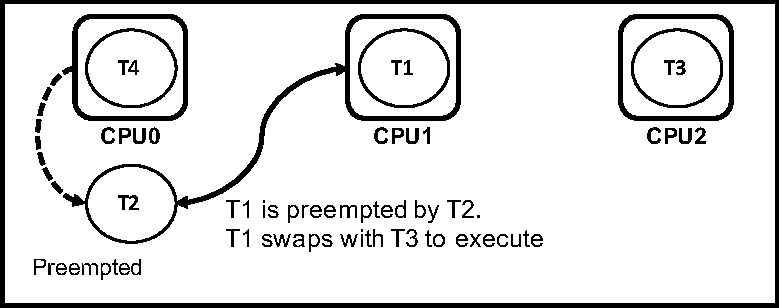
\includegraphics[width=.6\columnwidth]{graphics/swap1.pdf}}
\subfigure[] {\label{swap2}
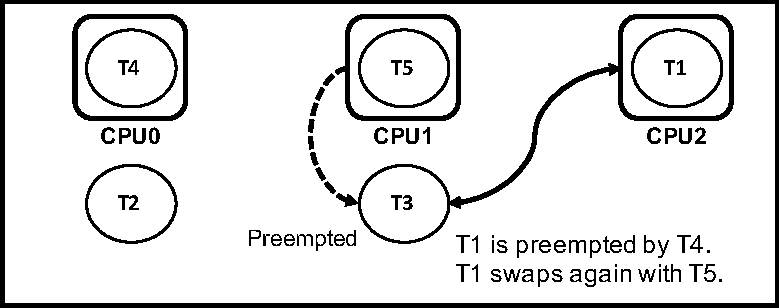
\includegraphics[width=.6\columnwidth]{graphics/swap2.pdf}}
\caption{Nested preemption in task swapping approach.}
\label{nestedpreemptiontaskswapping}
\end{figure}

The swapping approach seems to carry high overheads as extra migrations are introduced. However, as the migrations during a swapping is performed should be lower than expected. The task swapping approach has the advantages.
\begin{itemize}
\item No modifications to the scheduler is required.
\item Once the helping task swaps with holder, it can pull the holder back to the original processor if being preempted again without the need for extra mechanisms. 
\item As the helping task keeps spinning, it automatically prevents the release of lower priority tasks without the need for a ceiling facility.
\item While migrating, the holder can execute with the ceiling instead of a higher priority as the spinning task is migrated away.
\end{itemize}
However, the swapping approach brings a considerably high complexity to the MrsP implementation. In addition, as the pulling operation is modelled independent to the scheduler and cannot obtain a consistent snapshot of ready queues while migrating the holder, false migrations can still occur in this implementation.

\section{Preemption Queue With Non-Preemptive Sections (MrsP-NP)}
\label{Subsectionpreemptionqueue}
As mentioned before, false migrations undermines the efficiency of MrsP helping mechanism by either triggering extra migrations or missing required migrations. In addition, a migrated holder can be preempted immediately after being helped and resumed. When applying MrsP to a system where high priority tasks are released frequently, the resource holder can suffer from frequent migrations even if false migrations are prevented. As a result, it is possible that the holder spends much more time migrating rather than executing, which greatly undermine the usability of the protocol. To avoid the migration issues and to achieve a high efficiency while helping a preempted holder, the Preemption Queue with Non-Preemptive Sections approach is developed, as described below. 

To guarantee that each migration decision is valid, two rules are proposed while building the helping mechanism:
\begin{enumerate}
\renewcommand{\labelenumi}{(\theenumi)}
\item The helping mechanism should be built by pull operations only.
\item The migration decisions made by the protocol should be modelled as scheduling decisions.
\end{enumerate}
There are three concerns with the push operation:
\begin{itemize}
\item The push operation suffers from ineradicable race conditions. Due to the limitation of the partitioned run-queue structure, it is not possible to get a consistent states of multiple run-queues unless obtaining all run-queue locks.
\item Even with unlimited push attempts, tasks need to travel through all the potential suitable processors between the source partition and the target partition. Instead, this can be achieved via pull operations by one migration.
\item As scheduling decisions are made independently on each processor, it is not possible to model a migration decision made by push to a local scheduling decision of a remote processor.
\end{itemize}
Due to these concerns, push operations should not be adopted for MrsP implementation so that only pull operations can be applied. To solve the race conditions with the local run queue, we require that the pull operation needs to be modelled inside the scheduler and as a part of scheduling decision. Accordingly, during each reschedule point, the pull operation will be triggered if the to-be-scheduled task is spinning for a MrsP resource while the resource holder is being preempted. The scheduler then overrides the to-be-scheduled task by the preempted resource holder and passes it to Linux infrastructure to execute. With such an approach, the migrated task is eligible to execute as it is a scheduling decision while any newly released high priority tasks needs to wait for the next reschedule point. To avoid the need for acquiring multiple run-queue locks, a separate preemption queue can be adopted for storing preempted tasks with MrsP resources.

\begin{figure}[!h]
\centering
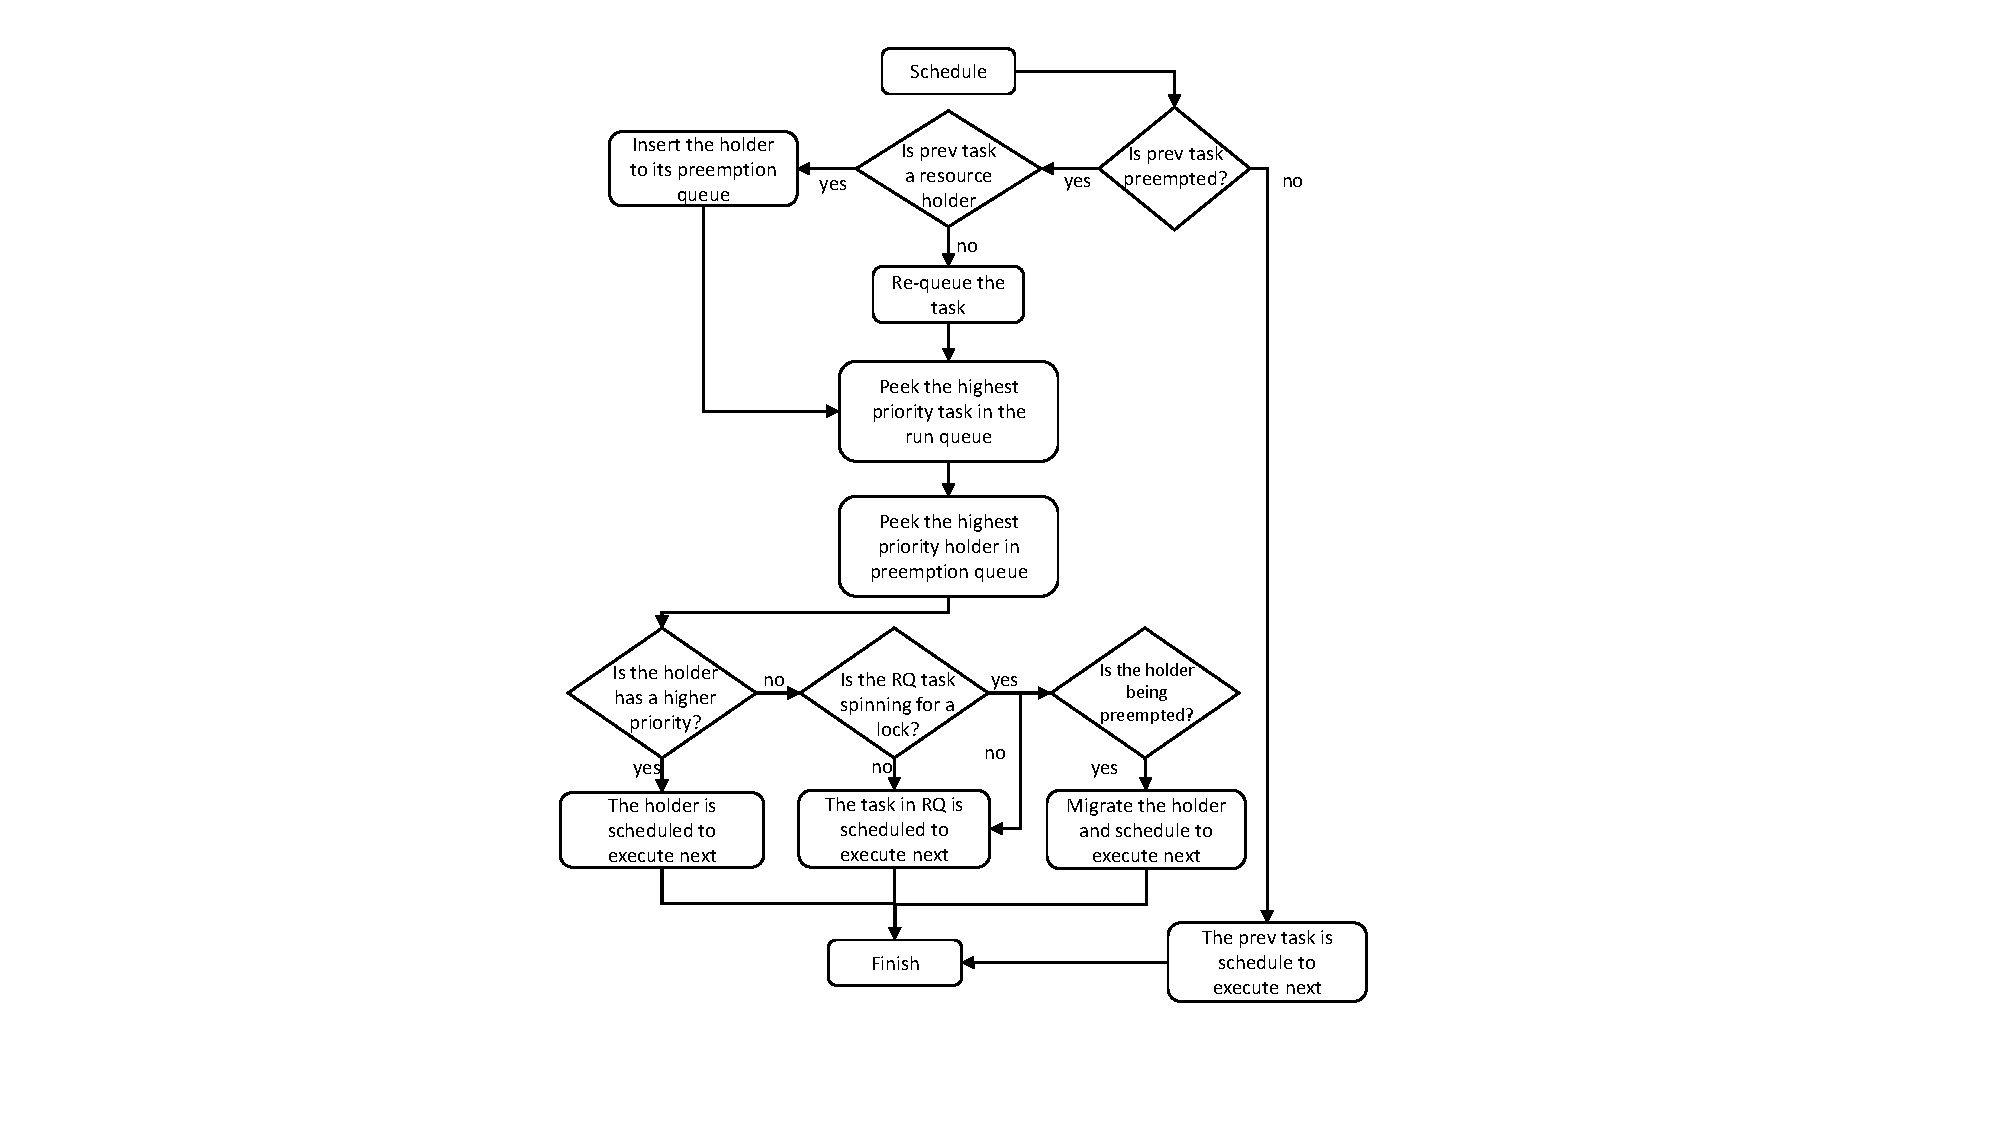
\includegraphics[width=.7\columnwidth]{graphics/pfp.pdf}
\caption{Scheduling sequence in modified P-FP scheduler}
\label{schedulingroutinepfp}
\end{figure}

The rules requires, the QP-NP version is implemented by pull operations only, and is built as part of the scheduling routine i.e. inside the scheduler. Upon each scheduling point, the pull operation checks whether the to-be-scheduled task is spinning for a MrsP resource and whether the resource holder is currently being preempted. If so, the scheduler pulls the holder with a slightly higher priority so that it can preempt the spinning task. However, such design idea raises two implementation issues.
\begin{enumerate}
\renewcommand{\labelenumi}{(\theenumi)}
\item While migrating the holder inside the scheduler, the run queue lock of the holder's processor should be acquired, which leads to a nested access of run queue locks and can cause potential deadlocks.
\item Upon a nested preemption, the task cannot migrates back to its original processor even if the preempter finishes as the scheduler cannot track the status of a task which migrated away and push operations are not allowed.
\end{enumerate}

To resolve the issues above, a preemption queue ($PQ$) is introduced in each processor. Once a holder is preempted, it will be placed into the $PQ$ of its original processor (even if the task is on a remote CPU). Each $PQ$ is protected with a local spin lock and its length is the same as the run queue's. Accordingly, the scheduler will look into the local $PQ$ to check whether a preempted holder is eligible to execute besides scheduling tasks in the run queue ($RQ$). During execution, a task will be inserted into its $PQ$ if:
\begin{itemize}
\item the scheduler identifies a higher priority task in the $RQ$ that is ready to execute while the task is running with a MrsP resource.
\item the spinning task is being preempted while waiting its turn to acquire the resource.
\end{itemize}
In addition, a preempted holder will be removed from the $PQ$ when:
\begin{itemize}
\item the scheduler picks the task in the $PQ$ to execute after the preempter finishes;
\item the task is pulled to a remote processor where a task is spinning for the resource.
\end{itemize}


By doing the above, the task is able to resume on its original processor in the nested preemption case. Figure~\ref{schedulingroutinepfp} depicts the scheduling routine of the modified P-FP scheduler with preemption queues. Upon a scheduling point, the scheduler first checks whether the previous scheduled task is preempted with a MrsP lock. If so, the holder will be placed in its $PQ$ with the corresponding ceiling priority. If the task is preempted without a MrsP lock, it will be re-queued into either the run queue or wait queue based on its execution state. The scheduler then looks into its $RQ$ and $PQ$ to check the highest priority tasks in both queues. The resource holder in $PQ$ will be scheduled to execute next if holds the highest priority. Otherwise, the task in the $RQ$ will be considered. However, if the task is spinning for a MrsP resource while the holder is being preempted on a remote processor, the pull operation will be triggered to remove the holder from its $PQ$ and migrate it here to execute. If the previous scheduled task is not preempted, it is allowed to keep executing.

By adopting such a facility, we realise the required functionalities defined in the protocol. Meanwhile, we can avoid the nested access between $RQ$ locks as well as the $PQ$ locks. As the locks of $PQ$s needs to be acquired inside the scheduler i.e. after obtaining the $RQ$ lock, no deadlocks will occur because no circular access can be formed. Yet it seems that the cost for a scheduling decision can be prolonged as the scheduler may need to compete for the $PQ$ locks. However, such competition only occurs if a scheduler is trying to pull a preempted holder with its currently scheduled task spinning for a resource.

To avoid frequent migrations of a resource holder and to improve the efficiency of the helping mechanism, we integrate MrsP with a short non-preemptive section to offer a trade-off between the maximum number of migrations a holder can suffer and bounding the resulting blocking on high priority tasks. Upon each migration, the resource holder is allowed to execute non-preemptively for a short period before it inherit the ceiling priority on the current partition. Accordingly, any newly released high priority tasks have to cope the cost of one NP section before it can preempt the holder and execute.

Accordingly, after migration, the holder will be assigned with the priority 0 (which is reserved by Litmus for priority boosting) so that it can execute effectively non-preemptively. To restore the corresponding ceiling priority of the holder after the NP section, one high resolution timer (\texttt{hrtimer}) is introduced for each on-line processors. A \texttt{hrtimer} will be initialized during the initialization phase of P-FP scheduler and will be armed each time when a holder is migrated to its partition due to preemption. When the timer triggers, it restore the holder's priority to the corresponding resource ceiling on current partition and invoke the scheduler to check whether a higher priority task is ready to execute. If the holder finishes the critical section (i.e. enters into \texttt{unlock} function) during the NP section, it disarms the timer first before realising the lock and migrating back. 

\section{Summary}
In this section, three approaches for implementing the MrsP migration-based helping mechanism inside kernel with fully partitioned scheduler are presented and discussed. Among the described approaches, the generic Linux migration approach carries the most straightforward design and implementation. The task swapping approach does not require modifications to the scheduler and does not need extra facility to prevent the execution of lower priority tasks after the holder migrated. However, these two implementations suffers from the false migrations and have the possibility that the holder spends more time migrating rather than executing. The PQ-NP implementation prevents both side effects by introducing the preemption queues and short non-preemptive sections.

\chapter{MrsP -- Outside-Kernel}
\label{Out Kernel}
The implementations we presented above are developed inside the Litmus kernel, which does not support affinity sets due to false migrations concerns. However, MrsP implementation can be extremely complex without the support of a migration facility. In this section we provide an outside-kernel MrsP implementation under a generic Linux system. With Linux, the helping mechanism can be realised simply by manipulating the affinity sets of tasks. In this chapter, we present an outside-kernel MrsP implementation developed based on the description of the prototype in the MrsP paper~\cite{burns2013schedulability}. 

The outside kernel implementation is built entirely though POSIX interfaces. The FIFO spin access is realised through a simple ticket facility and an affinity set is introduced to each MrsP lock struct. If a task requests a resource, it raises its priority to the ceiling, adds its processor to the resource affinity and spins on the resources to wait for its turn. Once the resource is granted, the task inherits the affinity of the resource during the period of accessing. Accordingly, Linux is responsible to handle the situation where the holder is preempted and to choose a suitable processor for migration. The following code illustrate the lock routine.
\begin{lstlisting}
int mrsp_lock(mrsp_lock lock) {
	int ticket;
	/* Set Ceiling priority and add processor to resource affinity*/
	pthread_setschedprio(pthread_self(), lock->prio_per_cpu[original_cpu]);
	CPU_SET(original_cpu, &lock->resource_affinity);
	
	atomic{
		/* update the affinity head (if not null), Otherwise we are the head.*/
		if (lock->head)
			pthread_setaffinity_np(lock->head, sizeof(cpu_set_t), &lock->resource_affinity);
		/* get a ticket*/
		ticket = lock->next_ticket;
		lock->next_ticket++;
	}
	
	while (1) {
		/* we now become the header */
		if (lock->owner_ticket == ticket) {
			atomic{
				/* set the head, update the resource affinity and raise the priority by 1. */
				lock->head = pthread_self();
				pthread_setaffinity_np(lock->head, sizeof(cpu_set_t),&lock->resource_affinity);
				pthread_setschedprio(lock->head, lock->prio_per_cpu[original_cpu] + 1);
				break;
			}
		}
	}
	return 0;
}
\end{lstlisting}

When the task releases the resource i.e. enters into \texttt{mrsp\_unlock()}, it removes its processor from the resource affinity, restores its original priority and affinities, and then returns from \texttt{unlock}, as shown in the pseudo code below:

\begin{lstlisting}
int mrsp_unlock(mrsp_lock lock) {
	cpu_set_t mask;

	/* the calling thread should hold the lock */
	if (pthread_self() != lock->head) 
		return -1;

	/* remove the processor from resource ceiling and increment the owner_ticket */
	atomic{
		CPU_CLR(original_cpu, lock->&resource_affinity);
		lock->owner_ticket++;
		lock->head = NULL;
	}

	/* restore task affinity and priority*/
	CPU_ZERO(&mask);
	CPU_SET(orinigal_cpu, &mask);
	pthread_setaffinity_np(pthread_self(), sizeof(cpu_set_t), &mask);
	pthread_setschedprio(pthread_self(), original_priority);

	return 0;
}
\end{lstlisting}




The outside-kernel version is the most simple and straightforward implementation among all the implementations proposed in this report due to the support from task affinities. However, besides the false migration and frequent migration issue, the frequent invoking of system calls can introduce extra overheads, which undermines the usability of the protocol.



\chapter{Conclusion}
\label{Conclusion}
In this report we investigate and explore feasible approaches to implement the MrsP migration-based helping mechanism under fully partitioned systems inside the kernel. We first present the commonly adopted approach for building such a helping mechanism: the generic Linux migration approach. This approach is straightforward to design and implementing but requires a huge modification to the scheduling routine i.e. the \texttt{finish\_switch()} function, which is invoked at the end of each scheduling decision. In addition, this approach suffers from false and frequent migration. Then two novel implementation approaches are proposed: the task swapping approach and the  preemption queue with non-preemptive sections approach. The major advantages carried by the swapping approach are (1) requires no modification to the scheduler and (2) requires no extra facility to prevent the execution of low priority tasks after the holder is migrated. However, the swapping approach does not avoid the migration problems. To prevent the migration problems and to achieve a higher efficiency, the MrsP-NP implementation is proposed by introducing preemption queues and non-preemptive sections. With the preemption queues, the pull operation can be fully integrated into the scheduling decision so that the false migrations are prevented. In addition, by introducing short non-preemptive sections to migrated resource holders, frequent migrations can be avoided and the holder can suffer from less migrations while accessing the resource. These features can be crucial to the efficiency and usability of the protocol when applied to fully partitioned systems. Finally we present an MrsP outside-kernel implementation under generic Linux, which also can suffer false and frequent migrations.


\bibliographystyle{abbrv}
\bibliography{ref}




\end{document}


